\label{background}
\obnote{The lit. review is required for a proper scholarly treatment of the subject. 
Background/Related Work should contain a literature review of other approaches for analyzing MD trajectories on HPC: 
at a minimum: VMD, HiMach, cpptraj (and pytraj), possibly mdtraj ? read the papers/websites and check for benchmarks. Look for others 
(Giannis already mentioned some in his paper and/or the workshop draft).}
\mknote{Giannis, Overal we need more references on here. In addition you mention the features of the library, but we need to point out the strength and weakness
of each library and make them bold. Maybe a Table like what you have added in ICPP paper on the comparison of frameworks that you mention what are their differences and how they
differ from each other will be good to be added here as well. Could you please add that to this section?}
\gpnote{First, I do not think this is the correct related work for this paper. Both frameworks here are using parallel reads and parallelize trajectory analysis. Also, I think this related work nullifies the paper. I suggest a related work closer to the workshop paper we were working.}
\mknote{Ok maybe we can have a look. But I do not think that they nullify this paper. What are your reasonings for this? Their approach is different. Does HiMach nullify CPPTraj approach? They are both discussing parallel analysis on MD trajectories?
Instead we can emphasize on the differences and strength of ours}
\mknote{I have another idea. We can compare the performance of cpptraj with our approach for two cases of large and small tcomp/tIO. Especially we can see if cpptraj can be scaled when tcomp/tIo is small (i.e. I/O bound jobs)}

CPPTraj~\cite{cpptraj-2013} offers three levels of parallelization. The two are through MPI and the third through OpenMP.
The MPI types of parallelization CPPTraj supports are show in Figure~\ref{fig:cpptraj_arch}. In more detail,
CCPTraj allows the parallel read between frames of the same trajectory or ensemble members of
the same trajectory. When it is used to analyze a single trajectory, all frames of the trajectory
are equally distributed over the number of MPI process that are used. Each process reads the frames
that are assigned to it, executes and writes the results of all processes to the same output file.
When ensemble mode is used, each ensemble member is assigned to an MPI process. As a consequence,
there have to be as many MPI processes as ensemble members. The user has the ability to increase 
CPPTraj's throughput by assigning more than one MPI processes per ensemble member. Each ensemble 
member is divided further the same way as a single trajectory.
\begin{figure}[ht!]
		\begin{subfigure}{.5\textwidth}
		\centering
		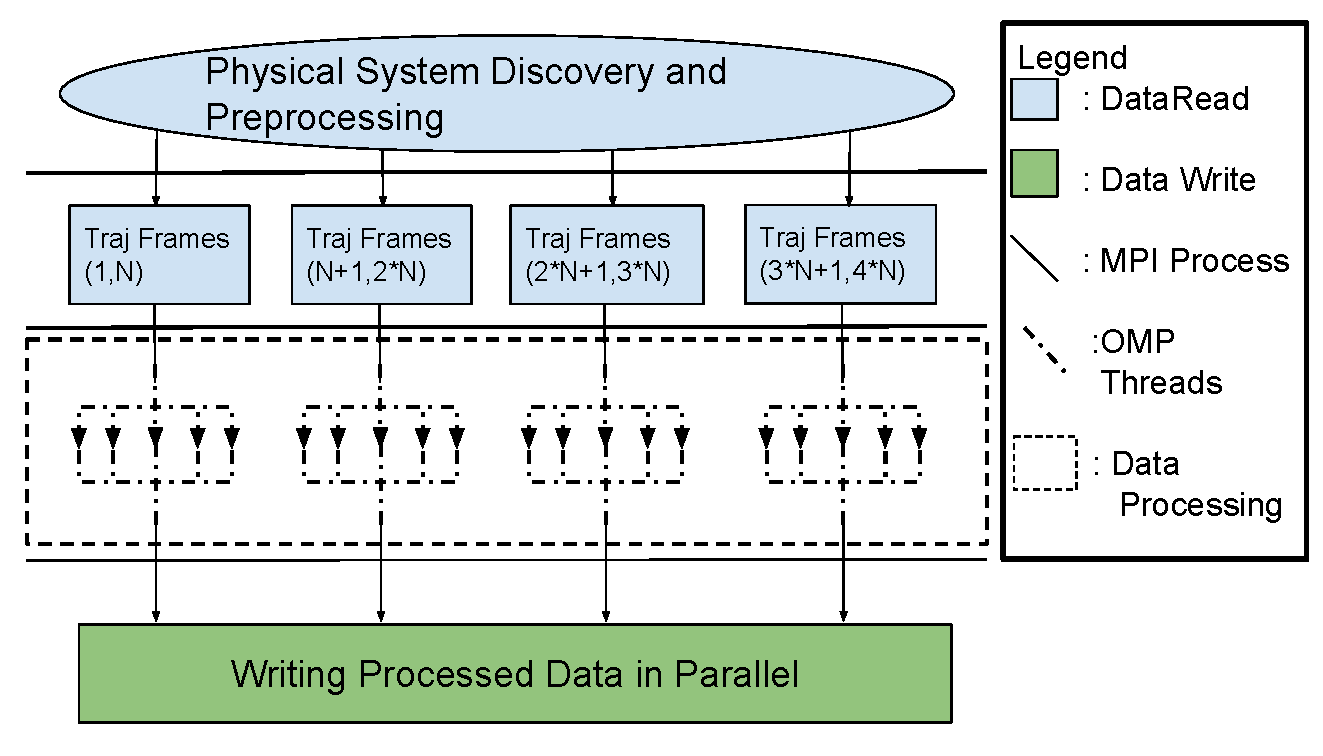
\includegraphics[width=.95\textwidth]{figures/CPPTrajExecutionSchematicSingleTrajectory.pdf}
	\end{subfigure}
	\begin{subfigure}{.5\textwidth}
		\centering
		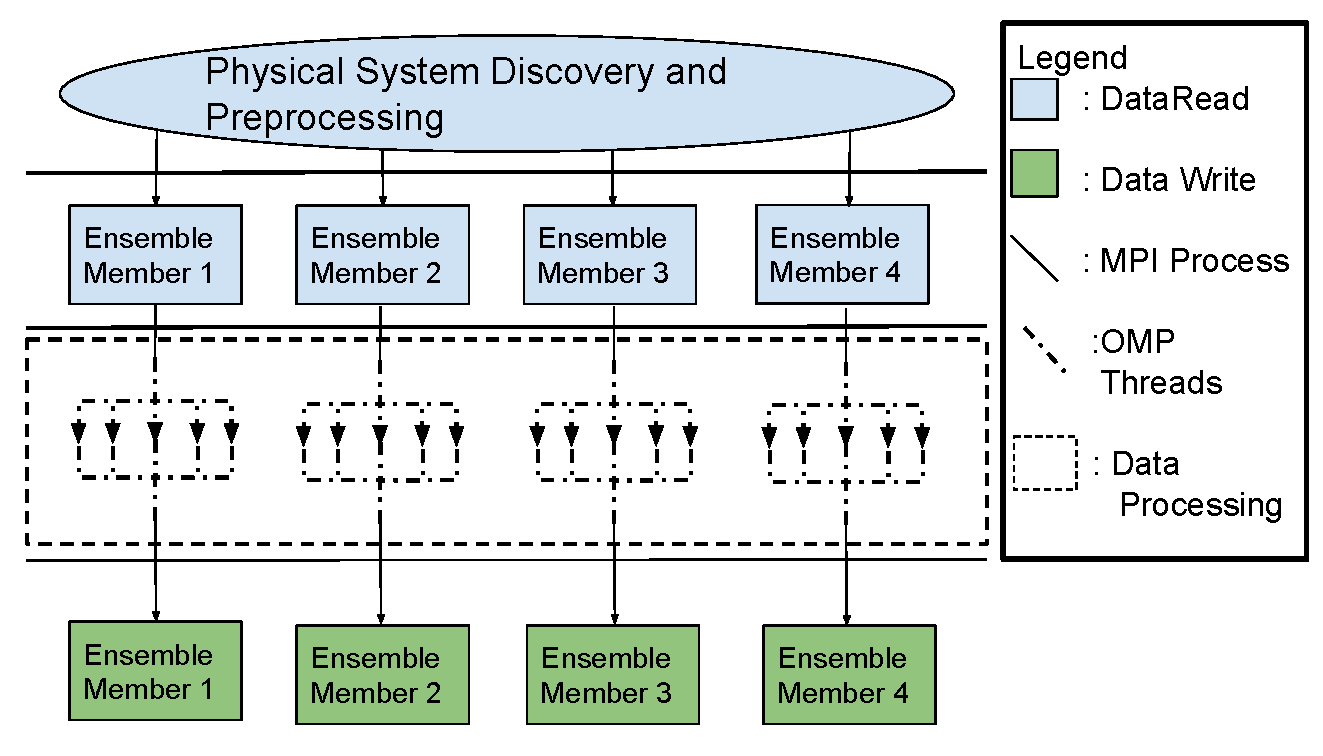
\includegraphics[width=.95\linewidth]{figures/CPPTrajExecutionSchematicEnsembleTrajectories.pdf}
	\end{subfigure}
	\caption{CPPTraj MPI modes of execution. The right figure shows the case where a single trajectory is
		given. The left figure shows the case where an ensemble of trajectories are given for analysis}
	\label{fig:cpptraj_arch}
\end{figure}

HiMach~\cite{himach-2008} was developed by D.E.Shaw Research group to provide a parallel analysis
framework for molecular dynamics simulations. HiMach extends Google's MapReduce
to provide a scalable API for MD trajectory analysis. HiMach API provides a series
of Python classes that are used to define trajectories, do per frame data acquisition
(Map class) and cross-frame analysis (Reduce class). After the user has defined all 
the above, HiMach's runtime is responsible to parallelize and distribute the Map and 
Reduce classes to the assigned cores. Data transfers between Map and Reduce phases are
done through a communication protocol created specifically for HiMach and it is transparent
from the user.